\documentclass{standalone}
\usepackage{tikz}

\begin{document}

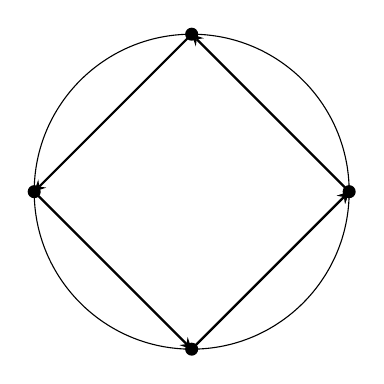
\begin{tikzpicture}[scale=2]
    % Draw the circle
    \draw (0,0) circle (1);

    % Define the points on the circle
    \foreach \i in {0, 90, 180, 270} {
        \node[fill=black,circle,scale=0.5] at (\i:1) {};
        \coordinate (P\i) at (\i:1);
    }

    % Draw the arrows
    \draw[-stealth, thick] (P0) -- node[midway, above] {} (P90);
    \draw[-stealth, thick] (P90) -- node[midway, right] {} (P180);
    \draw[-stealth, thick] (P180) -- node[midway, below] {} (P270);
    \draw[-stealth, thick] (P270) -- node[midway, left] {} (P0);

    % Connect the last point back to the first for completeness
    \draw[-stealth, thick] (P270) -- (P0);
\end{tikzpicture}

\end{document}